\chapter{User Manual}
\label{ch:manual}
This chapter will have the user manual. These UI/UX elements are crafted to be responsive and visually appealing, ensuring a seamless and enjoyable experience for users as they practice medical procedures and scenarios.
\section{Choose Scenario}
The user interface (UI) enhances the user experience (UX) with intuitive design elements. Users start by selecting a scenario corresponding to a patient's medical issue from a menu of various conditions or scenarios.
\begin{figure}[h]
    \centering
    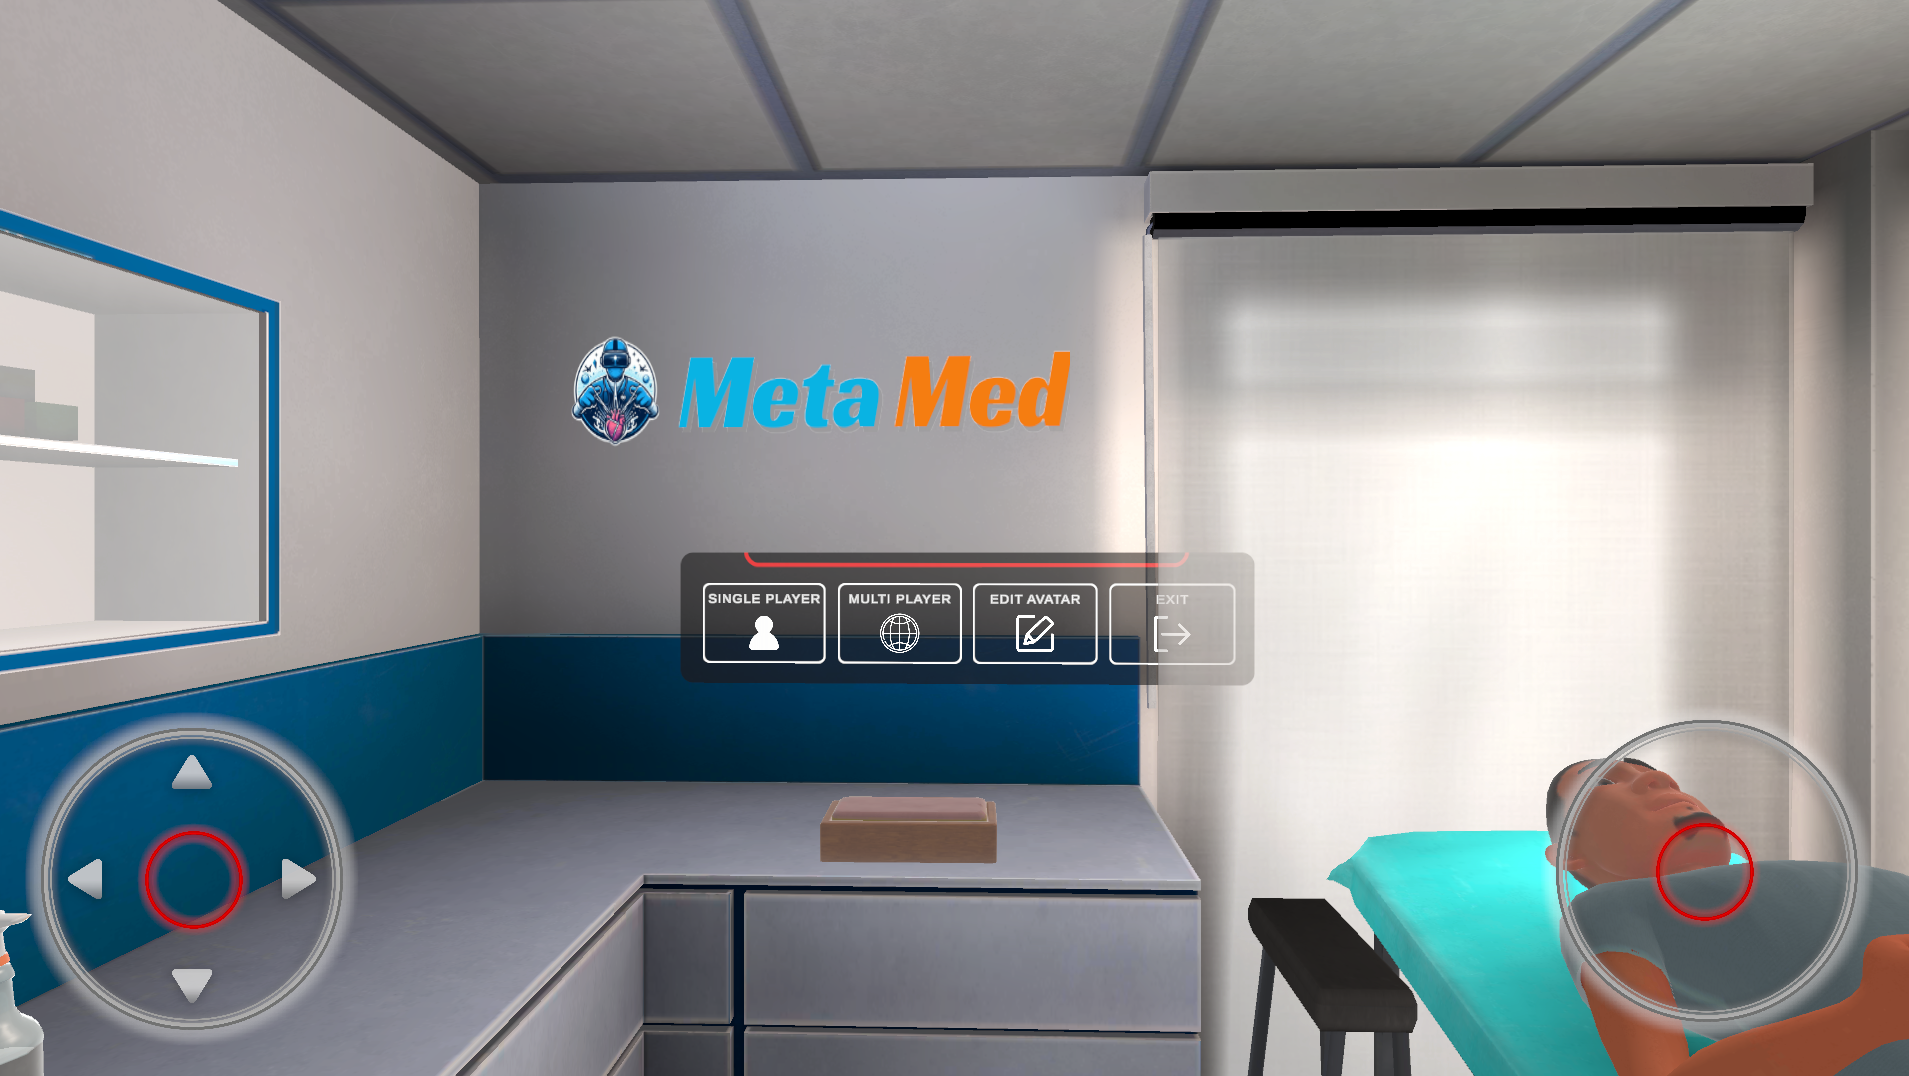
\includegraphics[width=0.7\textwidth, height=0.3\textheight]{Images/User Manual.png}
    \caption{User Manual}
    \label{fig:User Manual}
\end{figure}

\section{1.1 Start Session}
Once a scenario is chosen, the UI features a 1.1 toggle menu for keyboard interaction, enhancing user \begin{figure}[h]
	\centering
	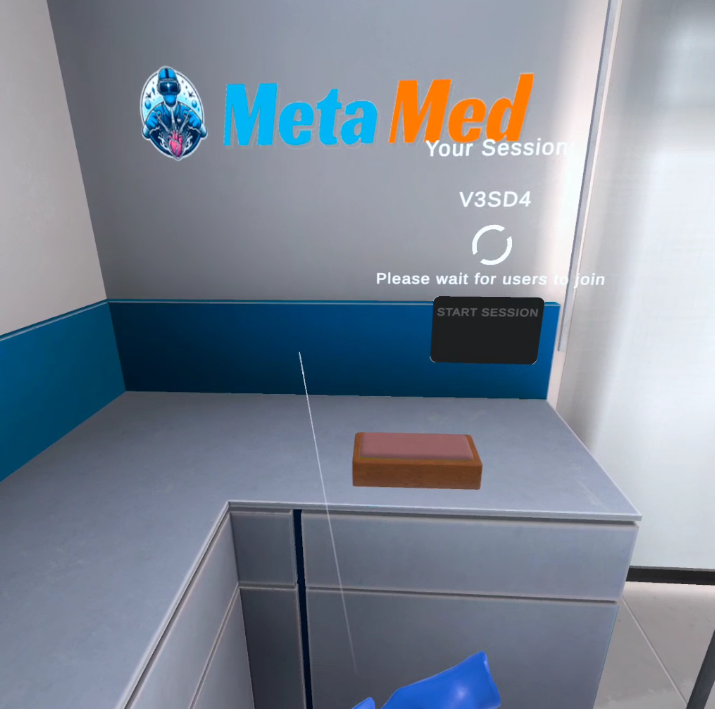
\includegraphics[width=0.7\textwidth, height=0.3\textheight]{Images/start session.png}
	\caption{Start Session}
	\label{fig:Start Session}
\end{figure}

\section{1.2 Choose Scenario}
Here can choose scenario like operation of leg, arm, foot etc.
\begin{figure}[h]
	\centering
	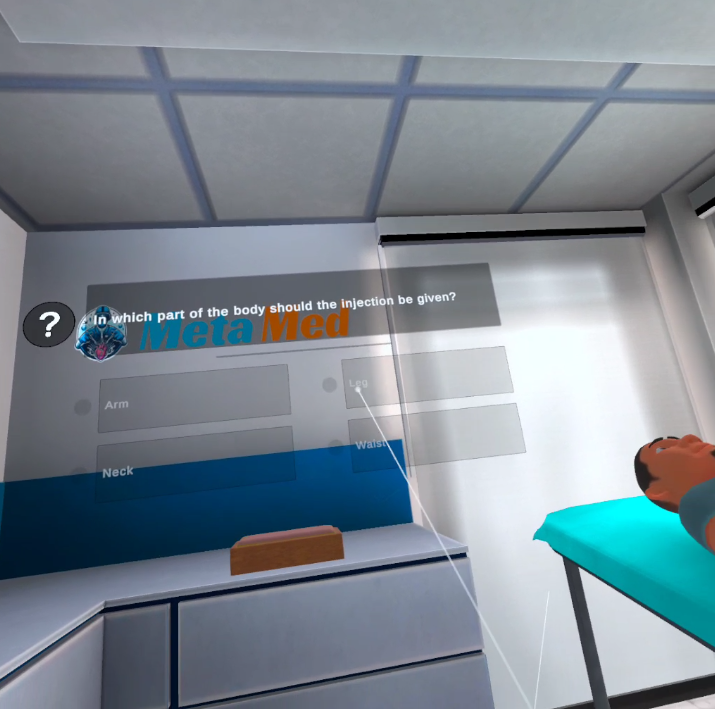
\includegraphics[width=0.7\textwidth, height=0.3\textheight]{Images/select body part.png}
	\caption{Choose Scenario}
	\label{fig:ChooseScenario}
\end{figure}